\label{chuong_2}

\section{Kiến trúc tổng thể hệ thống}

Hệ thống được thiết kế theo mô hình kiến trúc AIoT định hướng biên, tập trung vào khả năng xử lý tại chỗ nhằm đảm bảo tính thời gian thực. Cấu trúc hệ thống được chia thành bốn tầng chức năng chính để thuận tiện cho việc quản lý và mở rộng (Hình \ref{fig:system_architecture}).

\begin{figure}[p]
    \centering
    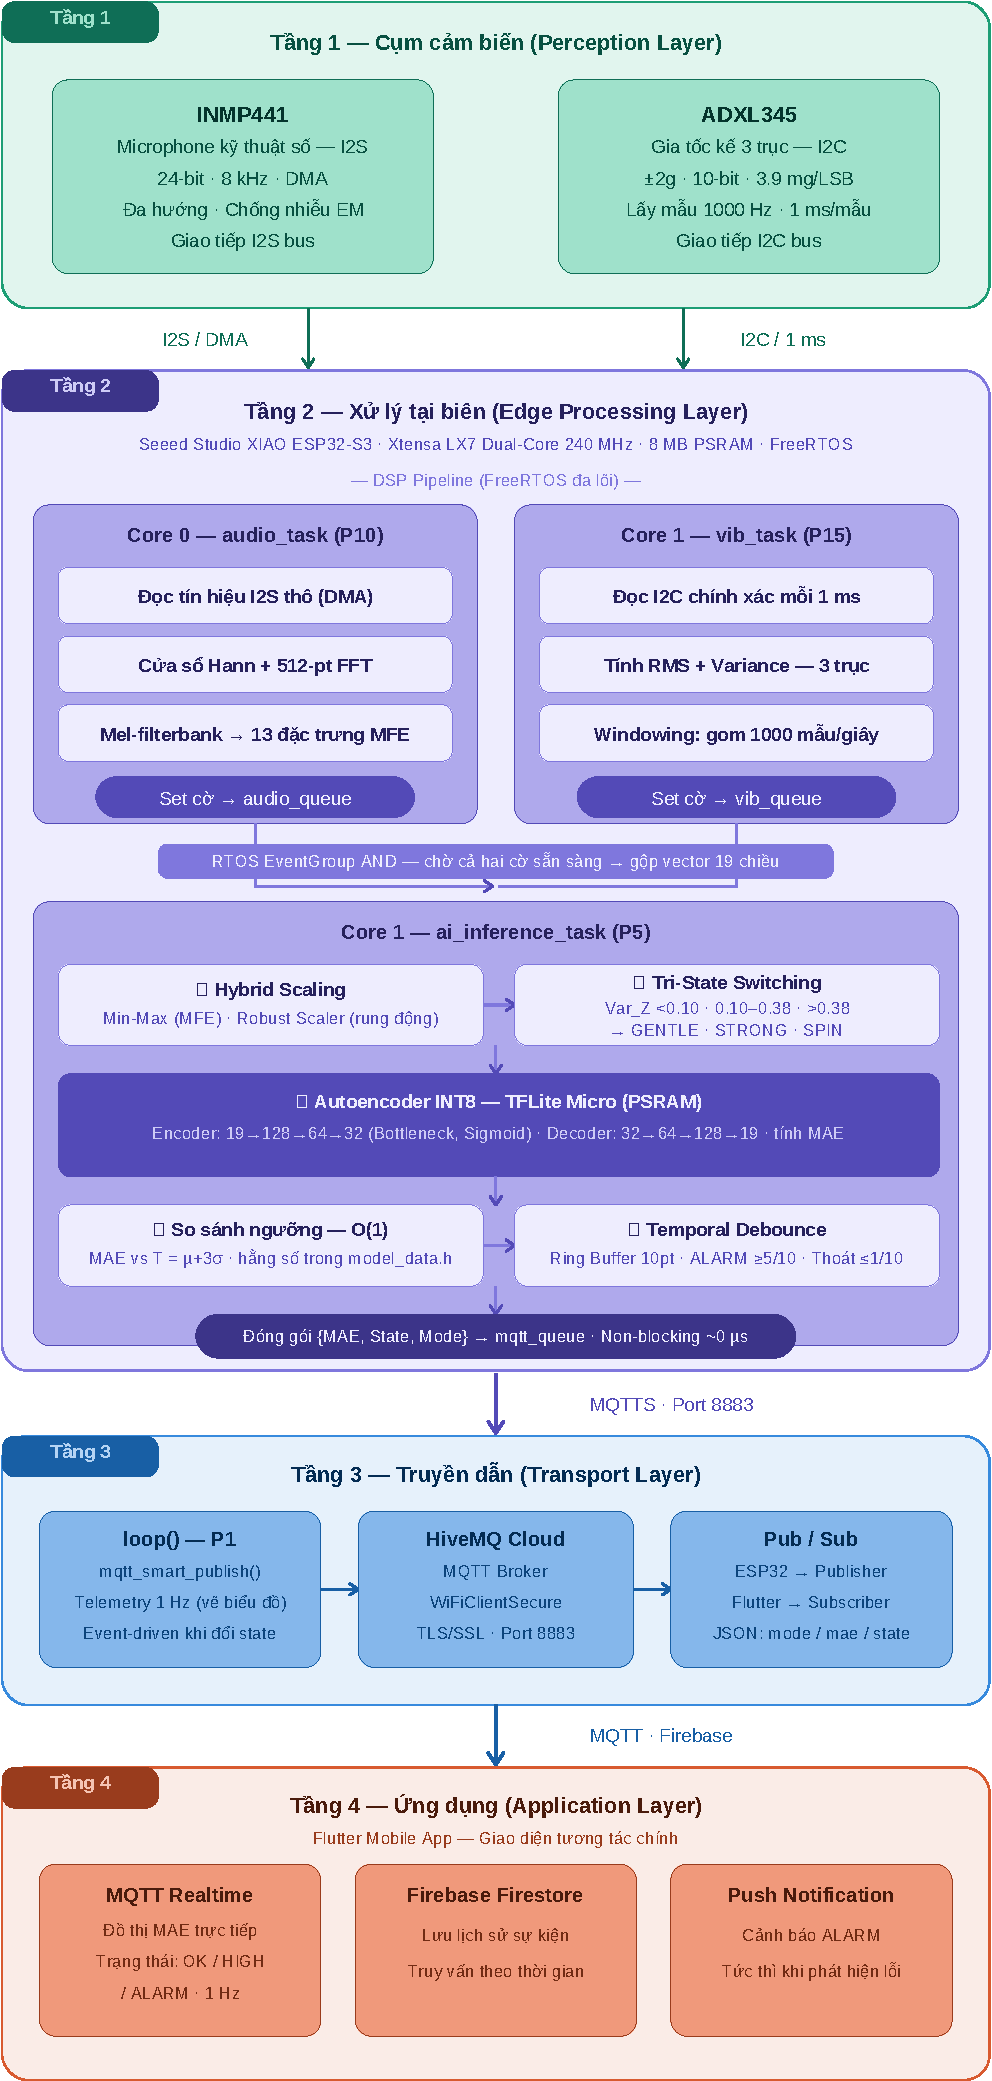
\includegraphics[width=0.65\linewidth]{chap2/image/kien_truc_4_tang_v4_cropped.pdf}
    \caption[Sơ đồ kiến trúc tổng thể hệ thống]{Sơ đồ kiến trúc tổng thể hệ thống bao gồm 4 tầng chức năng: Tầng cảm biến, Tầng xử lý tại biên, Tầng truyền dẫn và Tầng ứng dụng.}
    \label{fig:system_architecture}
\end{figure}

\subsection{Sơ đồ khối chức năng}

Các khối thành phần trong hệ thống tương tác theo luồng dữ liệu một chiều để tối ưu hóa thời gian phản hồi:

\begin{itemize}
    \item \textbf{Tầng cảm biến:} Gồm microphone kỹ thuật số INMP441 (I2S) thu tín hiệu âm thanh và cảm biến gia tốc ADXL345 (I2C) đo rung động cơ học của lồng giặt.
    
    \item \textbf{Tầng xử lý tại biên:} Sử dụng vi điều khiển Seeed Studio XIAO ESP32-S3 làm đơn vị xử lý trung tâm. Tại đây, dữ liệu thô được đưa qua đường ống xử lý tín hiệu số, trích xuất thành vector đặc trưng 19 chiều và nạp vào mô hình mạng nơ-ron tự mã hóa lượng tử hóa INT8 để suy luận \cite{ref_1_lord}. Hệ thống tận dụng kiến trúc lõi kép để thực hiện song song các tác vụ thu thập dữ liệu và tính toán mạng nơ-ron.
    
    \item \textbf{Tầng truyền dẫn:} Sử dụng giao thức MQTTS qua cổng 8883 để kết nối với HiveMQ Cloud. Đây là lớp trung gian điều phối thông tin từ thiết bị biên đến ứng dụng người dùng một cách bảo mật qua lớp mã hóa TLS/SSL.
    
    \item \textbf{Tầng ứng dụng:} Ứng dụng di động phát triển trên nền tảng Flutter đóng vai trò giao diện tương tác chính. Ứng dụng tích hợp đồng bộ dữ liệu thời gian thực qua MQTT và dữ liệu lịch sử qua Firebase Firestore. Cơ chế thông báo đẩy được sử dụng để cảnh báo người dùng kịp thời về các sự cố hỏng hóc.
\end{itemize}

\subsection{Đường ống xử lý luồng dữ liệu}

Quy trình xử lý dữ liệu được thiết kế theo cấu trúc luồng tuyến tính, đảm bảo tính toàn vẹn từ dữ liệu vật lý đến quyết định logic:

\begin{enumerate}
    \item Thu thập và Tiền xử lý: Tín hiệu âm thanh đi qua bộ lọc cửa sổ Hann và phép biến đổi Fourier nhanh 512 điểm để trích xuất 13 đặc trưng bộ lọc Mel. Song song đó, tín hiệu rung động (lấy mẫu ở tốc độ 1000 mẫu/giây) được tính toán giá trị hiệu dụng và phương sai để làm cơ sở phân tích trạng thái.
    
    \item Định tuyến trạng thái: Dựa trên phương sai trục Z của rung động, hệ thống tự động xác định máy đang vận hành ở pha nào (GENTLE, STRONG, hoặc SPIN). Từ đó, vi điều khiển thực hiện nạp và kích hoạt mô hình AI chuyên biệt tương ứng lên vùng đệm tensor.
    
    \item Suy luận AI và so sánh ngưỡng: Vector đặc trưng được đưa qua lớp chuẩn hóa kép trước khi vào mô hình mạng nơ-ron tự mã hóa để tính toán lỗi tái tạo (MAE). Hệ thống sử dụng các ngưỡng phát hiện dị thường đã được tối ưu hóa riêng biệt cho từng pha vận hành. Các giá trị này được nhúng trực tiếp dưới dạng hằng số tĩnh nhằm triệt tiêu độ trễ tính toán, cho phép nhận diện lỗi với độ phức tạp $\mathcal{O}(1)$.
    
    \item Hậu xử lý: Để triệt tiêu báo động giả do nhiễu cơ học tức thời, hệ thống áp dụng cơ chế bộ lọc cửa sổ trượt có nhớ và bộ đệm vòng lưu giữ 10 trạng thái gần nhất. Thuật toán trễ được tích hợp để thiết lập bộ quy tắc bất đối xứng: hệ thống chỉ chuyển sang trạng thái ALARM khi có ít nhất 5/10 mẫu vượt ngưỡng, và chỉ khôi phục về trạng thái bình thường khi tỷ lệ lỗi giảm xuống mức tối thiểu ($\le$ 1/10). Cơ chế có trạng thái này đảm bảo độ tin cậy tuyệt đối cho hệ thống.
\end{enumerate}

\subsection{Cơ chế điều phối đa nhiệm trên FreeRTOS}

Đồ án triển khai kiến trúc song song thực sự trên lõi kép của FreeRTOS nhằm triệt tiêu hiện tượng mất đồng bộ thời gian trong kỹ thuật kết hợp dữ liệu đa phương thức:

\begin{itemize}
    \item Lõi số 0: Chuyên trách tiền xử lý tín hiệu. Tác vụ audio\_task với mức ưu tiên 10 thực hiện đọc I2S và liên tục thực thi khối lệnh FFT/bộ lọc Mel nặng về tính toán dấu phẩy động.
    \item Lõi số 1: Đảm nhiệm hai tác vụ quan trọng. Tác vụ vib\_task được cấp đặc quyền cao nhất trong nhóm tác vụ người dùng với mức ưu tiên 15 nhằm đảm bảo chu kỳ lấy mẫu phần cứng I2C chính xác ở mức 1 ms. Tác vụ ai\_inference\_task với mức ưu tiên 5 chịu trách nhiệm vận hành mô hình TFLite Micro và chạy thuật toán phân tích cảnh báo.
\end{itemize}

Việc đồng bộ hóa giữa các lõi được thực thi qua cơ chế nhóm sự kiện (đảm bảo logic cổng AND - AI chỉ chạy khi cả hai cảm biến đã sẵn sàng) và hàng đợi luồng an toàn. Đặc biệt, hệ thống cô lập hoàn toàn khâu truyền dẫn mạng khỏi tiến trình AI. Tác vụ AI chỉ làm nhiệm vụ đóng gói cảnh báo và đẩy vào mqtt\_queue qua thao tác không chặn (mất $\sim$0 $\mu$s). Hàm loop() nội tại của vi điều khiển, chạy ngầm ở mức ưu tiên 1, đóng vai trò tiêu thụ dữ liệu từ hàng đợi này và xử lý các gián đoạn I/O mạng. Thiết kế này giúp triệt tiêu hoàn toàn rủi ro độ trễ mạng làm treo cứng tiến trình giám sát AI tại biên.

% ==============================================================================
% DANH MỤC TÀI LIỆU THAM KHẢO TRÍCH DẪN (CHI TIẾT CHO MỤC 2.1)
% Sao chép dòng dưới đây vào file .bib hoặc môi trường thebibliography của bạn
% ==============================================================================
% \bibitem{ref_1_lord} M. Lord, "TinyML Anomaly Detection," Master's thesis, Dept. Comput. Sci., California State Univ., Northridge, CA, USA, 2021.
